
\section*{Problem 1: Predicting Air Out Probability of Batted Balls}
\label{sec:p1}

\subsection{Data}
\label{subsec:data}

It is important that we carefully consider the structure of the provided data before making predictions of the air out probability. There are a couple of key non-linearities which I will discuss before diving into my modelling choices.

First, consider the horizontal exit angle. As shown in Figure \ref{fig:hist}, we have many observations for balls which are hit straight into foul territory. Naturally, all observed air outs fall within approximately 45 degrees of dead center, give or take a few degrees for balls caught in foul territory or balls which slice fair after leaving the bat. I account for this by including $horz\_exit\_angle$ as a 2nd-degree polynomial in all models.

\begin{figure}[htb]
  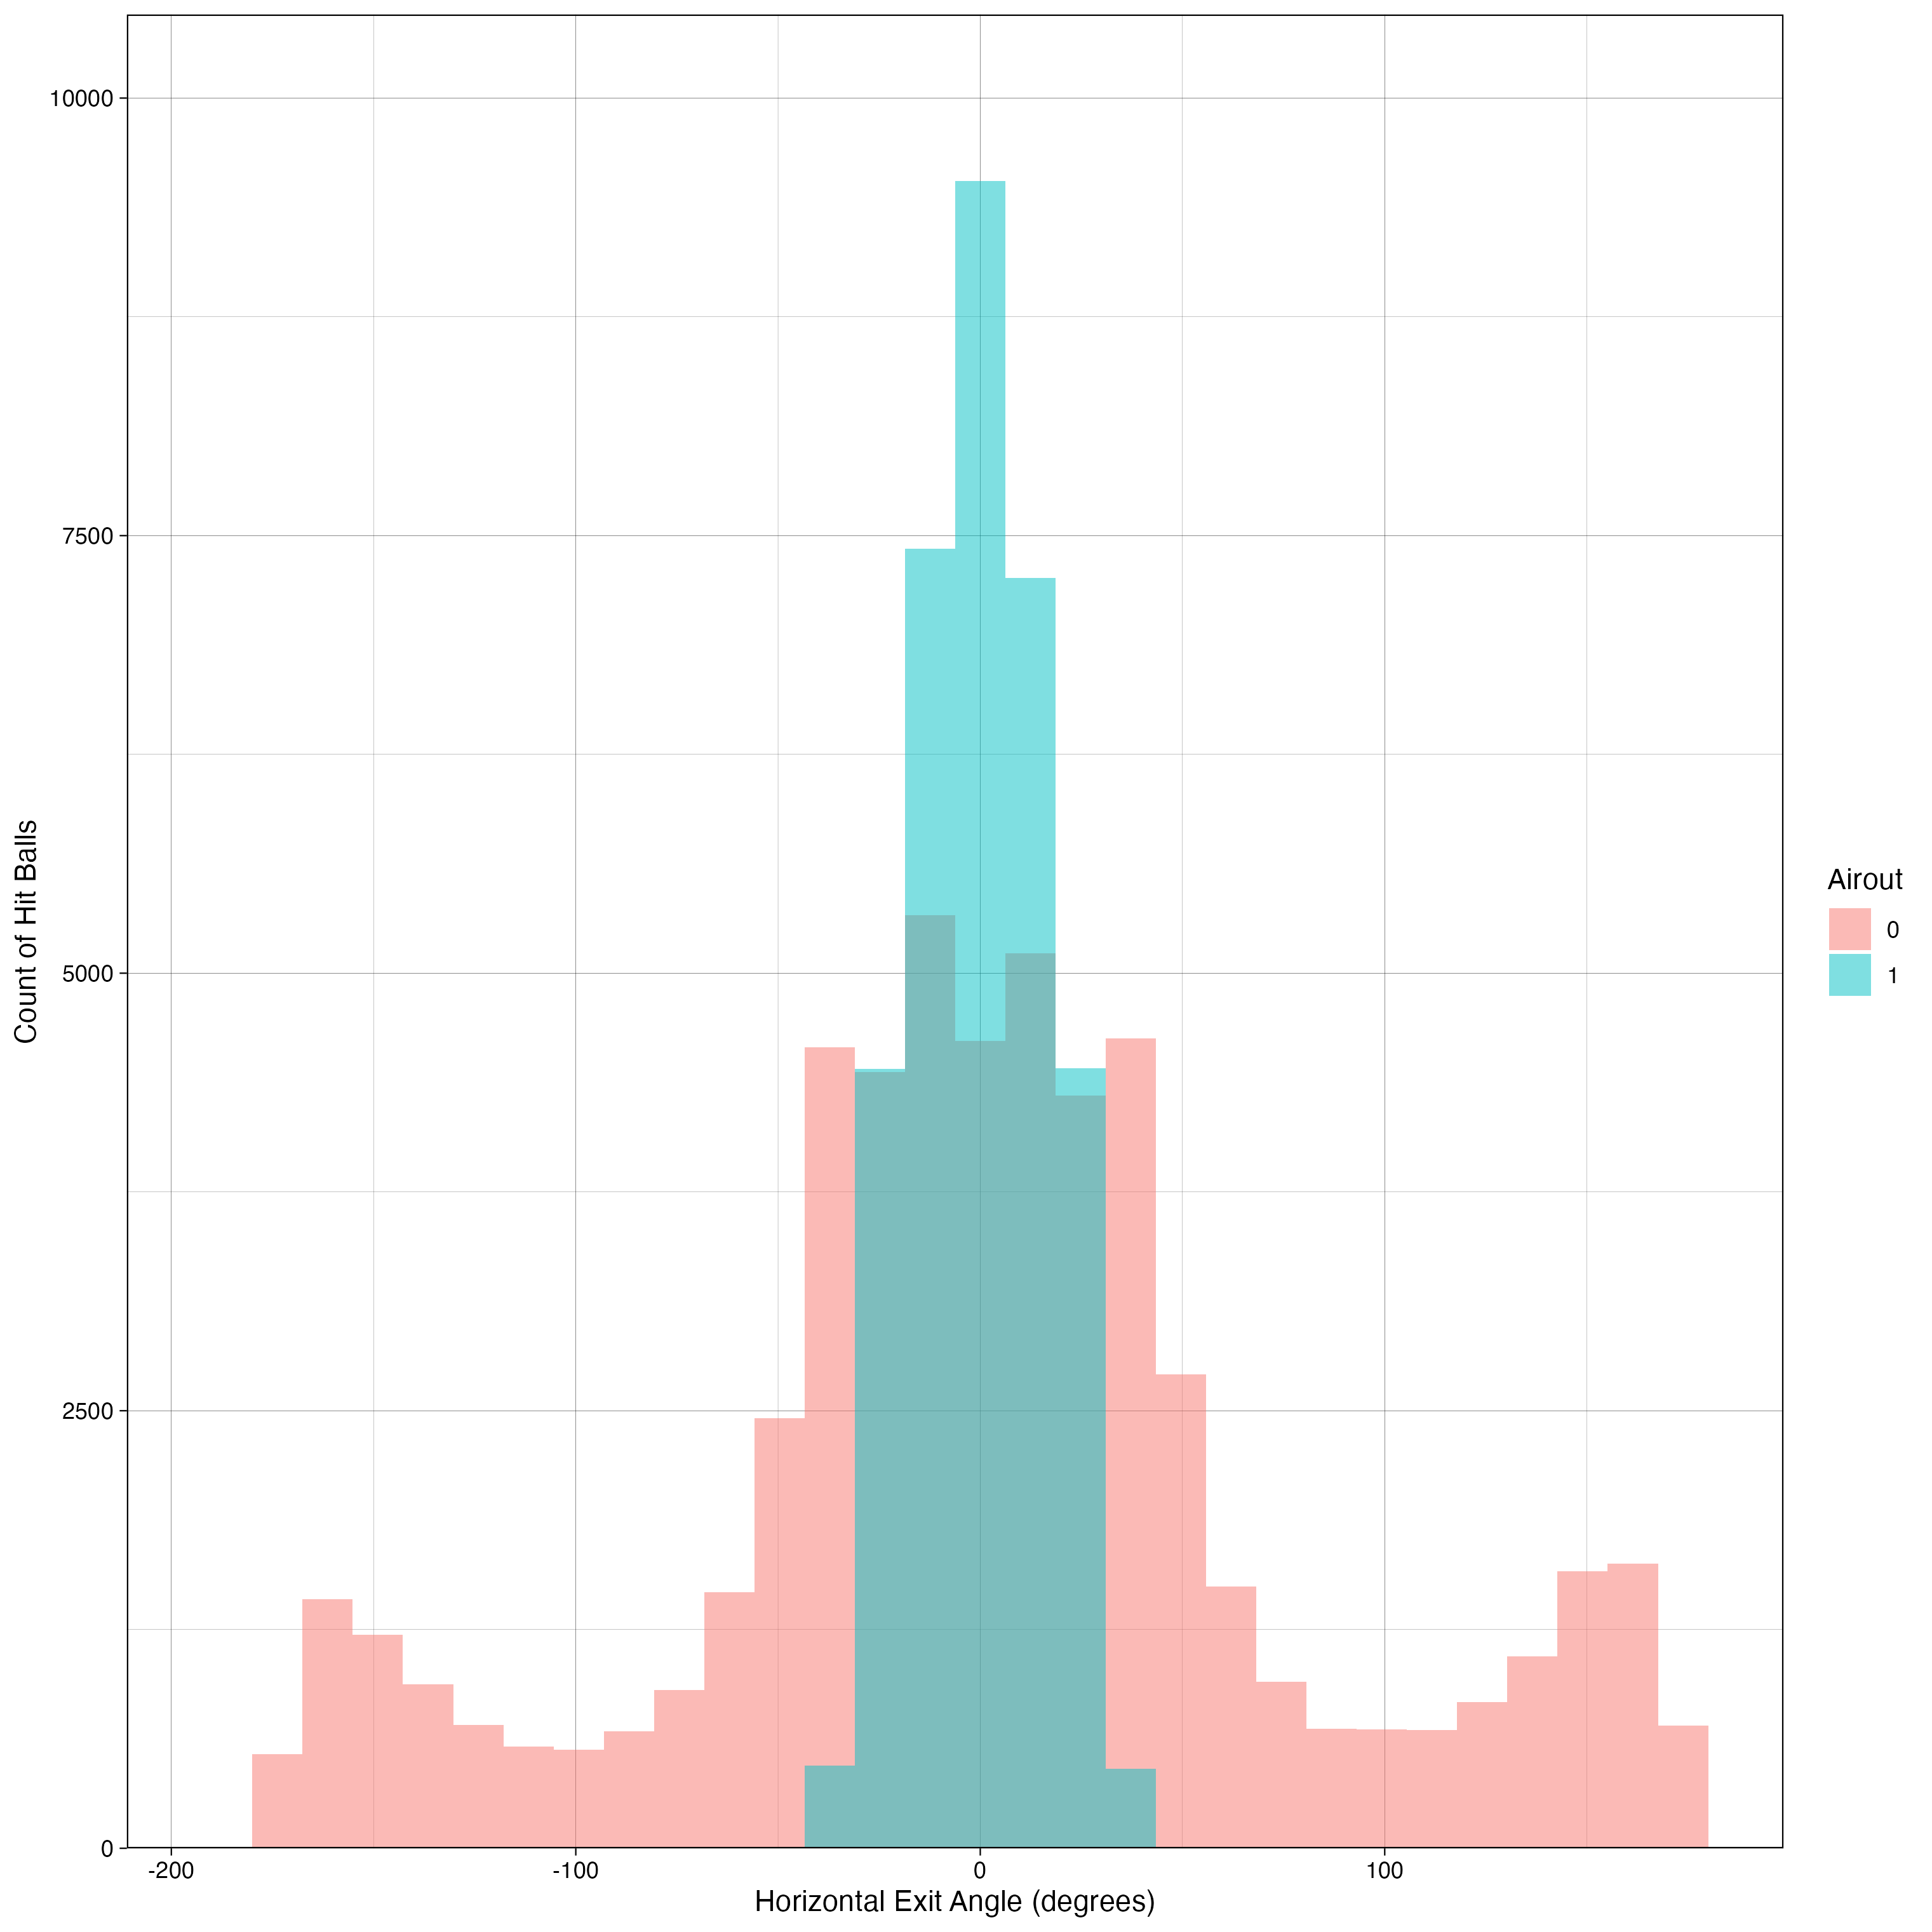
\includegraphics[width = 0.47\textwidth]{../../output/figs/horz_exit_angle_hist.png}
  \caption{Count of Hit Balls by Horizontal Exit Angle}
  \label{fig:hist}
\end{figure}

The key variables used to determine whether a fair ball is catchable by an outfielder are vertical exit angle and exit speed. Importantly, these two variables are more informative when combined. For instance, a ball hit at a relatively high exit angle but low exit speed is much more likely to be a fly out than a ball hit at the same exit angle but with a very high exit speed (which may end up in the bleachers instead).

I adapt the Statcast definition of a \textbf{barrel} to account for different types of hits. Specifically, I categorize hit balls into one of six categories based on a combination of exit angle and exit speed \cite{chamberlain}:

\begin{enumerate}
  \item Poorly hit (weak)
  \item Poorly hit (topped)
  \item Poorly hit (under)
  \item Flare or burner
  \item Solid contact
  \item Barreled
\end{enumerate}

The distribution of these hit types in the training data is shown in Figure \ref{fig:barreled}. Since the data has been pre-filtered to non-infield plays, we have no observations of poorly hit (weak) balls and only one observation of a poorly hit (topped) ball.

I apply a combination of theory and experimentation (via a 10-fold cross validation procedure) for feature selection. I exclude variables which:
\begin{enumerate}
  \item Have little theoretical justification for being included in the model, and
  \item Add nothing to the predictive power of the model when they are included.
\end{enumerate}
For example, the variable indicating if the hit occurred in the top or bottom of the inning is excluded from most models. There is no clear reason why this variable should affect air out probability, and including does not change the model's performance as measured by accuracy and log-loss score.

Unless mentioned otherwise, the variables included are: temperature, exit speed (and its square), hit spin rate, vertical exit angle, horizontal exit angle (and its square), a set of indicator variables corresponding to unique venues, and a set of indicator variables corresponding to the hit type variable (described above).

Note that hit spin rate has 1297 missing observations (out of 91,553). In the interest of maximizing the amount of training data available, I impute the missing values at the mean value of 2902.84.


\begin{figure}[htb]
  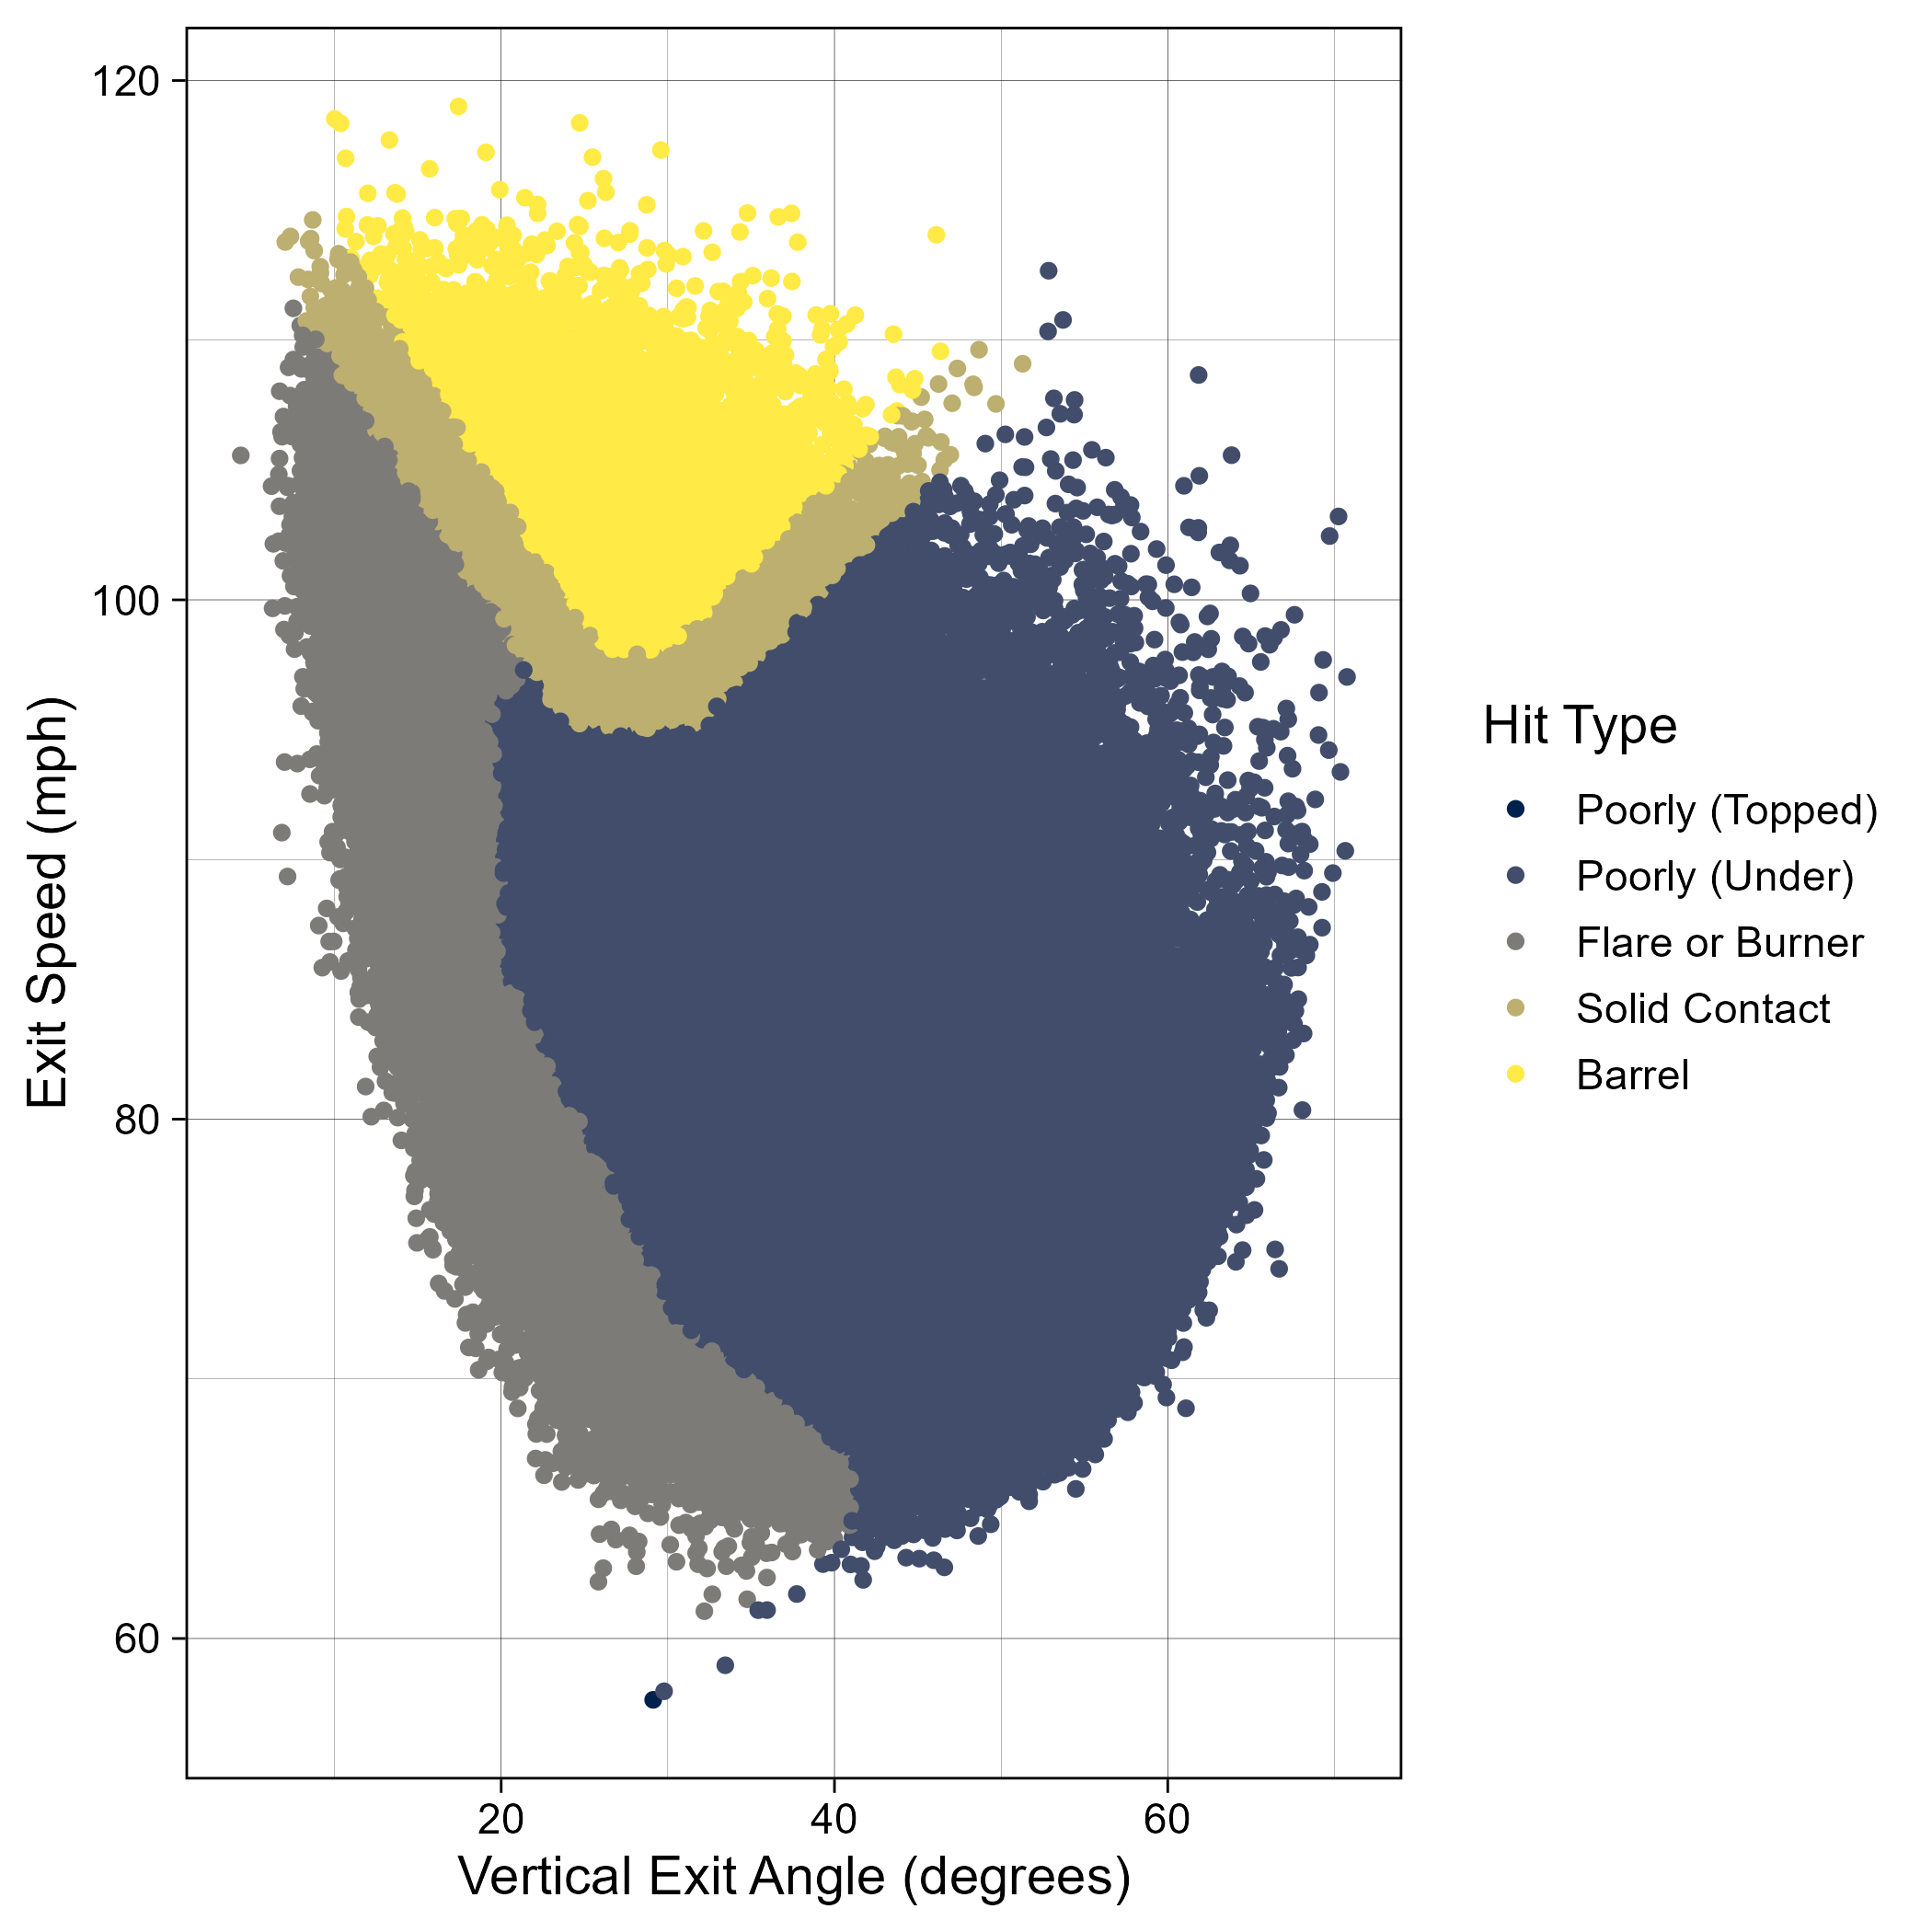
\includegraphics[width = 0.47\textwidth]{../../output/figs/barreled.png}
  \caption{Hit Type by Exit Speed and Vertical Exit Angle}
  \label{fig:barreled}
\end{figure}

\subsection{Modeling and Results}
\label{subsec:model}

I apply three different machine learning procedures to predict the probability of an air out in the test data: logistic classification, random forests, and a linear support vector classification (SVC) model.

\subsection{Extensions}
\label{subsec:results}

There are several ways I would expand upon the analysis presented here given more time and resources. First, I would be interested in incorporating more detailed location and weather data. Temperature is a good start, but I would like to tie each venue\_id and game date to local conditions including humidity, wind direction, wind speed, and if the venue is indoors.

Second, I would like to investigate hit spin rate in more detail. It is difficult to know how hit spin rate will affect the distance a ball travels, and thus the likelihood of an air out, without also knowing if it is backspin, topspin, or side spin.

Finally, incorporating data on player positioning could produce interesting results. This would likely also interact with the handedness of the batter and pitcher, increasing the amount of useful data I could incorporate into the model.